Campi Flegrei's unrest is recorded by ground displacement and seismicity. Tan et al. (2025) use a machine-learning-assisted earthquake catalog to resolve active structures and evaluate possible sources of unrest. Their study is observational: its central results describe the location, timing and character of earthquakes, rather than solutions of a coupled physical forward model. Here, the completed independent calculations are placed in the same scientific sequence. Published images are confined to the separate comparison PDF.

\section*{The current phase of unrest}
Figure 1 reconstructs the historical context from the explicitly permitted routine catalog and displacement observations and explicitly labeled historical source estimates. The routine snapshot contains 16,046 located events from 2005 through 20 March 2025, including five events with duration magnitude at least 4.0. Monthly counts include all routine events; the cumulative series includes 7,218 events with $M_d>0.2$. These external records are separate from the independently detected catalog.

The displacement reconstruction contains 128 historical entries (114 leveling surveys, 13 source-provided estimates and one source-provided reconstruction) and 8,743 daily GNSS observations through 20 March 2025. The original 1905--2023 interval is extended with observed data. A common vertical datum is obtained from overlapping observation records. The long sequence resolves subsidence, the major twentieth-century uplift episodes, and the recent uplift. It does not by itself distinguish magmatic from hydrothermal forcing. All three panels remain partial because the historical catalog snapshot, basemap and exact displacement-stitching convention differ or are incompletely specified.
\begin{figure}[H]
\centering
\par\smallskip\textbf{Panel 1A--C: partially reproduced}\par
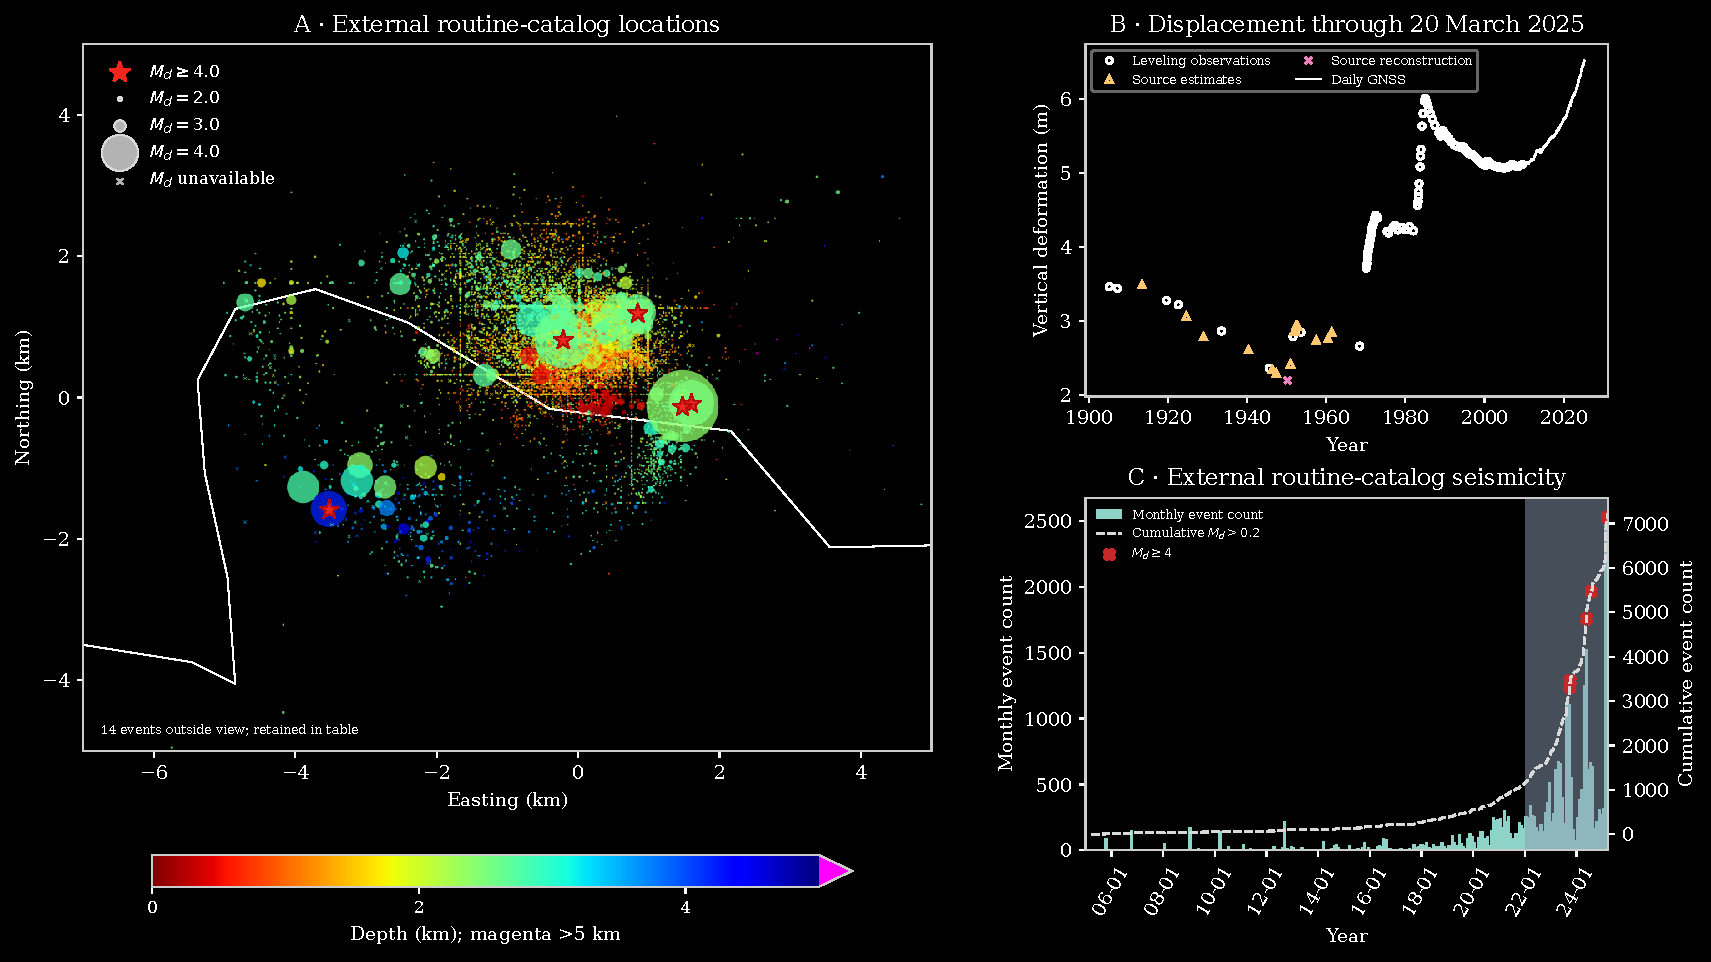
\includegraphics[width=.94\linewidth,height=.66\textheight,keepaspectratio]{figures/figure_1_combined.pdf}
\caption{Seismicity and ground displacement. Partial reconstruction from permitted original displacement observations and external routine-catalog records. A: 16,046 located routine events and five Md>=4 stars. B: historical leveling datum; daily GNSS through 20 March 2025, with the extension beyond 2023 shaded. C: all monthly counts and exact-time cumulative Md>0.2; March includes days 1--20 only. This is not the independently detected catalog. The basemap and live catalog snapshot differ from the publication.}
\label{publication:1}
\end{figure}


\section*{Improving the earthquake catalog}
Where two counterparts are shown, the first uses the frozen 1,015-association cohort and the second the latest 1,023-association cohort. They overlap and are not independent confirmations or additive event counts.

The current eligible continuous-observation checkpoint contains 246,668 picks and 3,271 provisional associations from 1,285 files and 13,467.933 channel-hours. 2996 associations have causal usable arrivals; 552 meet the numerical calibration selection. 1435 locations pass VELEST filters and 1050 remain after both TomoDD rounds and the gap filter. All known event-selected snippets are excluded. These calculations remain provisional; filter passage does not establish correct event identity or fault geometry.

\begin{figure}[H]
\centering
\missingresult{All panels/views}{Panels A and B require a multiyear calibrated, relocated catalog and magnitudes. Only nine provisional associations exist.}
\caption{Temporal evolution of seismicity. Seismicity rates by region and depth versus time are not reproduced.}
\label{publication:2}
\end{figure}


\section*{A clearer view of the current phase of unrest}
Figure 3 shows the 123 independently relocated trial events. Five lie deeper than 5 km and are retained with an over-range color. Their sparse, scattered distribution does not recover the ring fault or its proposed depth limits. Calibration-path differences reach 0.89 km in depth and conditional SVD errors reach 4 km; fault-scale interpretations are therefore premature. Figure 4 remains unreproduced because no event passes the attempted focal-mechanism constraints.
\setcounter{figure}{2}
\begin{figure}[H]
\centering
\par\smallskip\textbf{Panel 3; provisional numerical counterpart: partially reproduced}\par
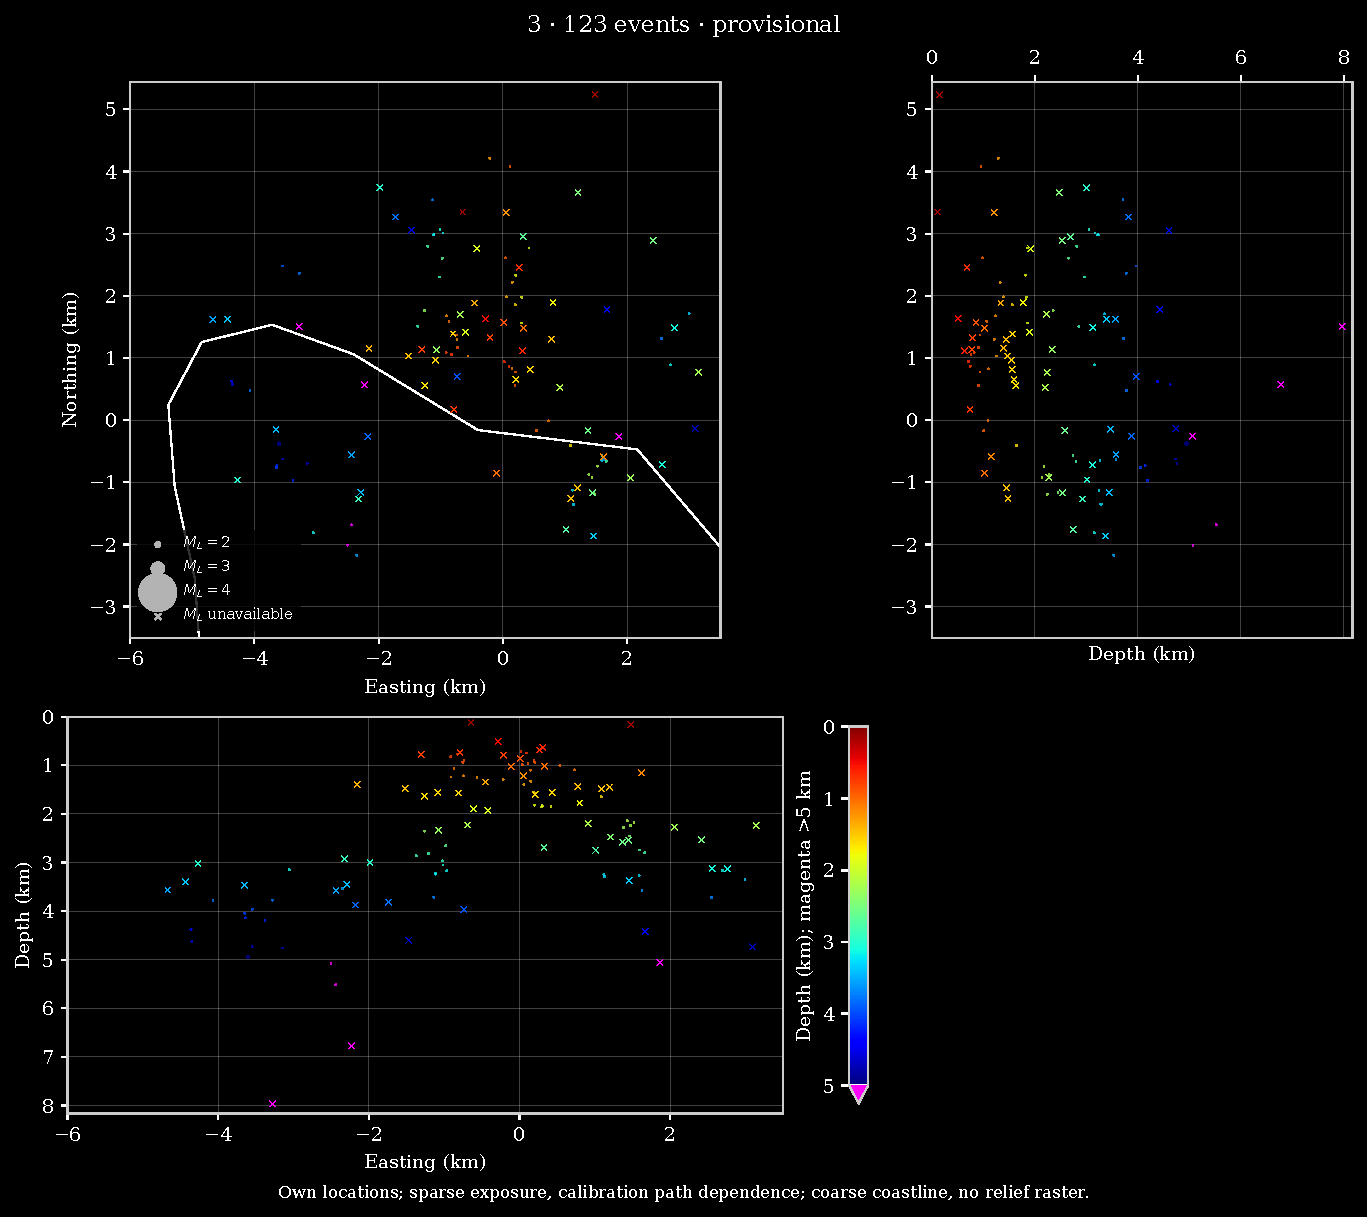
\includegraphics[width=.94\linewidth,height=0.310\textheight,keepaspectratio]{figures/figure_3_provisional.pdf}
\par\smallskip\textbf{Panel Latest extended cohort: independently rerun, provisional: partially reproduced}\par
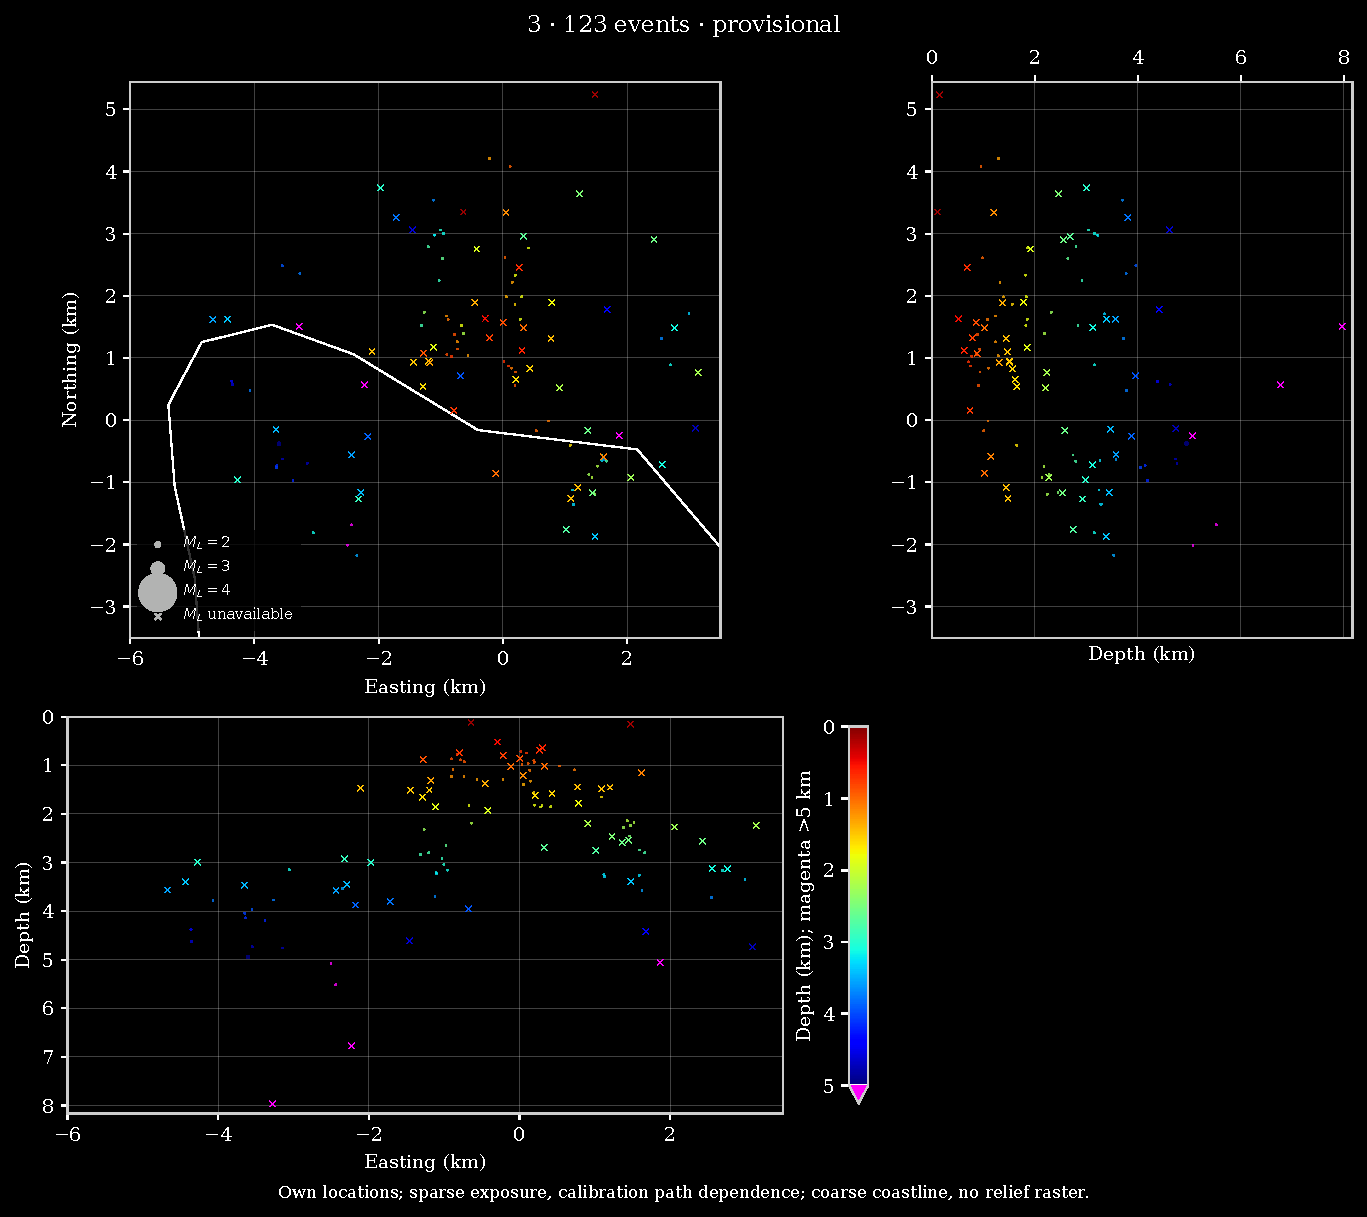
\includegraphics[width=.94\linewidth,height=0.310\textheight,keepaspectratio]{figures/figure_3_extension.pdf}
\caption{Spatial distribution of seismicity. 123 independently relocated trial events, 0.111--7.965 km depth. Own relative magnitudes set sizes where available; crosses mark missing magnitudes. This scattered subset does not establish the published ring or its depth limit. Provisional independent observations and processing; sparse coverage, unreviewed phases, calibration path sensitivity. Not established fault geometry or exact reproduction. The additional extended-cohort view uses separately numbered, independently rerun results. Magnitudes and SVD uncertainties were not inherited by integer event ID.}
\label{publication:3}
\end{figure}

\setcounter{figure}{3}
\begin{figure}[H]
\centering
\par\smallskip\textbf{Panel 4; current provisional independent calculation: partially reproduced}\par
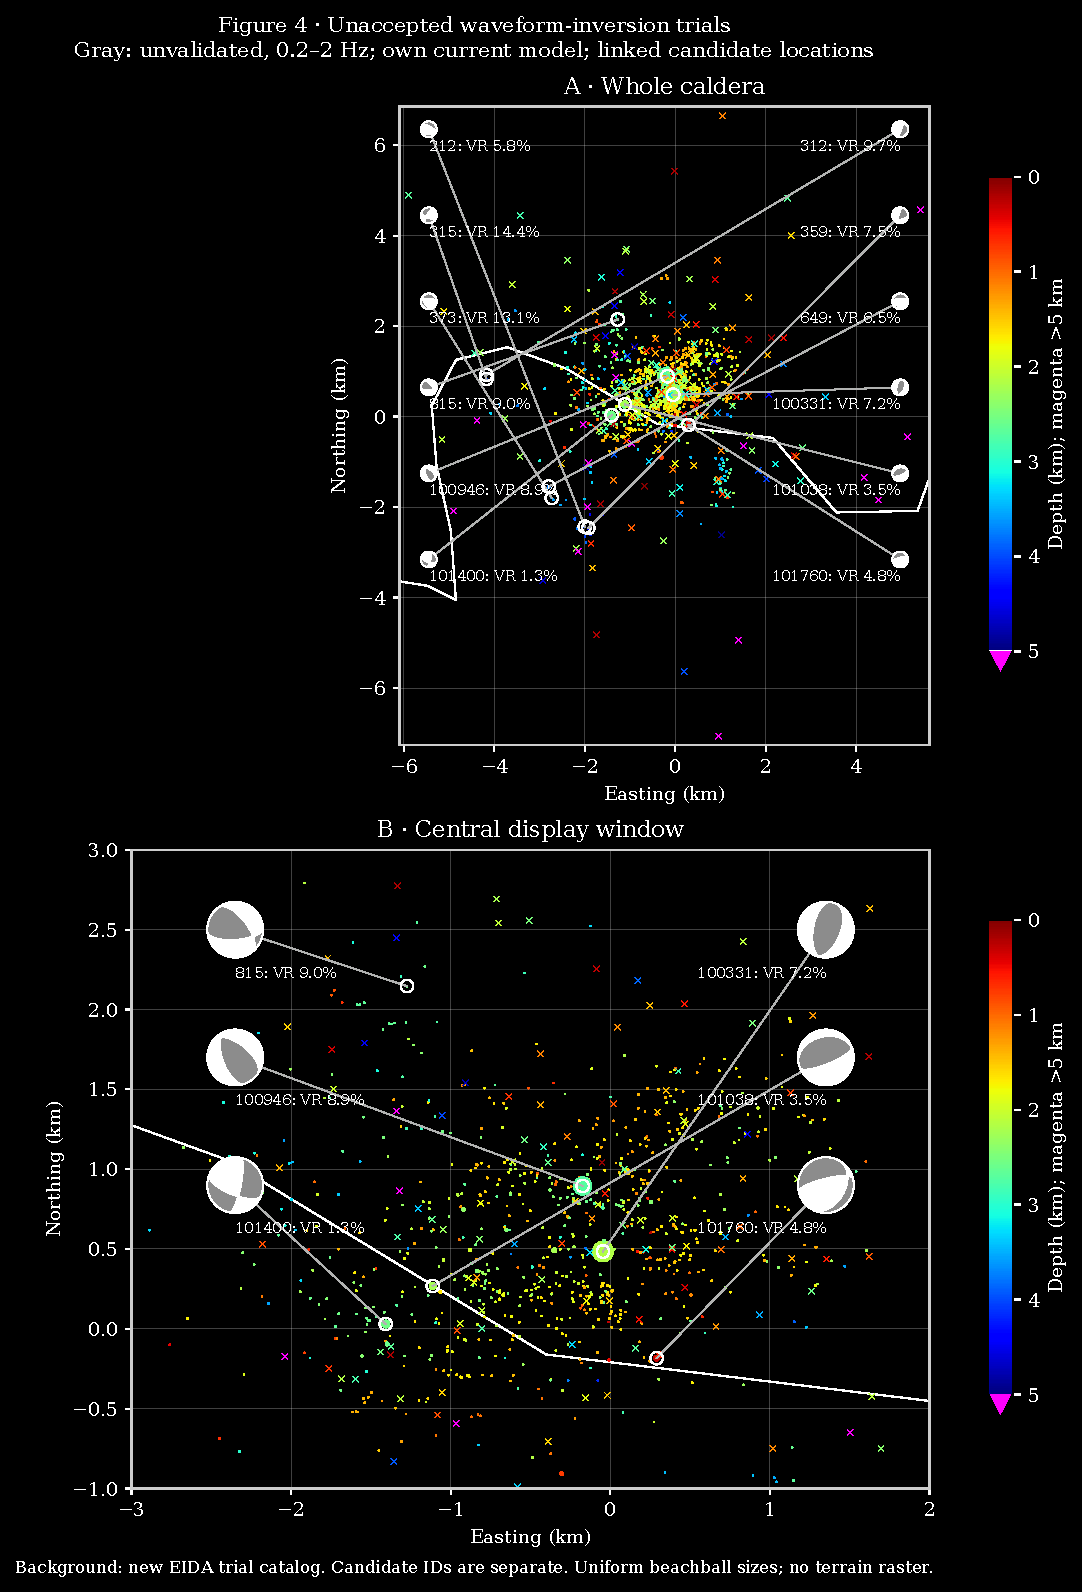
\includegraphics[width=.94\linewidth,height=0.620\textheight,keepaspectratio]{figures/figure_4_eida_followup.pdf}
\caption{Focal mechanisms of larger events. 12 unaccepted own FK/gCAP trial fits using newly available EIDA records and the current own model and explicitly linked own candidate geometry. 99 AI-reviewed polarities, 108 AI-reviewed ratios; no human review. SKHASH returns 2 solutions. Low-band variance reduction 1.3--14.4\%; orientations change 45.0--95.0 degrees between frequency bands. Gray beachballs denote unvalidated trials; background is the new independent catalog, never joined to candidates by integer ID. SKHASH returns 2 quality-D trials. No scientifically accepted mechanism. Partial/provisional: sparse observations, alternative association profile, unreviewed phases and unresolved model/location accuracy. Numerical generation is not agreement with the publication.}
\label{publication:4}
\end{figure}


\section*{Implications for the physical process driving the unrest}
The reconstructed hybrid-template example in Figure S15C is an independently processed waveform observation. The limited template search produced \CurrentHybridCandidates{} unconfirmed threshold crossings; it does not establish recurring hybrid families or their evolution. Neither this result nor the initial associations can test the publication's inference about the presence or absence of upward seismic migration. The partial displacement history also does not distinguish magmatic and hydrothermal forcing. Such an interpretation would require the unresolved spatial and source constraints above.

\section*{New perspectives for improved seismic risk assessment}
Fault geometry and a calibrated magnitude distribution are needed to connect this analysis to seismic risk. The pilot magnitude measurements have not established the multiyear magnitude-frequency distribution required for Figure S8. The current results therefore provide no revised estimate of event probabilities, damaging-event locations or source dimensions. Their supported contribution is restricted to the partial observational reconstructions shown here and in the supplement.
